\documentclass[aspectratio=169]{beamer}

% Tema visual (ver theme.tex)
% theme.tex — Configuracion visual de los slides 3DM
% Tema estandar Madrid (robusto, sin dependencias externas)

\usetheme{Madrid}
\usecolortheme{default}

% Paleta de colores consistente con el informe
\definecolor{mainblue}{RGB}{0,70,130}
\definecolor{accentred}{RGB}{180,30,30}
\definecolor{lightgray}{RGB}{240,240,240}

\setbeamercolor{frametitle}{bg=mainblue, fg=white}
\setbeamercolor{title}{bg=mainblue, fg=white}
\setbeamercolor{subtitle}{bg=mainblue, fg=white}
\setbeamercolor{author}{fg=black}
\setbeamercolor{structure}{fg=mainblue}
\setbeamercolor{block title}{bg=mainblue, fg=white}
\setbeamercolor{block body}{bg=lightgray}
\setbeamercolor{alerted text}{fg=accentred}

% Fuentes
\setbeamerfont{frametitle}{series=\bfseries, size=\large}
\setbeamerfont{title}{series=\bfseries, size=\Large}
\setbeamerfont{subtitle}{series=\normalfont, size=\normalsize}

% Pie de pagina: numero de frame en texto puro (evita nullfont)
\setbeamertemplate{footline}{%
  \hfill\usebeamercolor[fg]{footline}%
  \usebeamerfont{footline}%
  \textbf{\mbox{\insertframenumber}}%
  \hspace*{2ex}%
  \vspace*{1ex}%
}

% Eliminar botones de navegacion
\setbeamertemplate{navigation symbols}{}

% Separadores de items mas limpios
\setbeamertemplate{itemize item}{\color{mainblue}\textbullet}
\setbeamertemplate{itemize subitem}{\color{accentred}--}


% Paquetes necesarios
\usepackage[spanish]{babel}
\usepackage[utf8]{inputenc}
\usepackage[T1]{fontenc}
\usepackage{lmodern}
\usepackage{amsmath, amssymb}
\usepackage{booktabs}
\usepackage{graphicx}
\usepackage{tikz}

% Operadores matematicos reutilizados del informe
\DeclareMathOperator{\OPT}{OPT}

% Metadatos del documento
\title{3-Dimensional Matching}
\subtitle{Karp \#17 --- Trabajo Grupal Optimizaci\'on}
\author{Javier Far\'ias \and Uriel Navarrete \and Vicente Abarca}
\institute{Universidad Andr\'es Bello}
\date{Abril 2026}

\begin{document}

% ---- Portada ----
\begin{frame}
  \titlepage
\end{frame}

% ---- Slides reales (6) ----
% 02_problema.tex — Slide 2: Definicion del problema
\begin{frame}{Problema: 3-Dimensional Matching (Karp \#17)}

\begin{columns}[T]
\begin{column}{0.52\textwidth}
\textbf{Datos:}
\begin{itemize}
  \item Tres conjuntos $X, Y, Z$ con $|X|{=}|Y|{=}|Z|{=}n$
  \item Conjunto de tripletas $T \subseteq X \times Y \times Z$, $|T|{=}m$
\end{itemize}

\medskip
\textbf{Objetivo (max-3DM):}
Encontrar el mayor subconjunto $M \subseteq T$ tal que cada elemento aparece a lo sumo una vez en $M$.

\medskip
\textbf{Ejemplo} ($n{=}3$, $m{=}5$):
\begin{itemize}
  \item $M^* = \{(x_1,y_1,z_1),\,(x_2,y_2,z_2),\,(x_3,y_3,z_3)\}$
  \item $|M^*| = 3 = n$ \alert{(matching perfecto)}
\end{itemize}
\end{column}

\begin{column}{0.44\textwidth}
\begin{tikzpicture}[scale=0.82, every node/.style={font=\small}]
  % Nodos X (izquierda)
  \foreach \i/\label in {1/$x_1$, 2/$x_2$, 3/$x_3$} {
    \node[draw, circle, fill=blue!15, minimum size=20pt] (x\i) at (0, -\i*1.1+1.6) {\label};
  }
  % Nodos Y (centro)
  \foreach \i/\label in {1/$y_1$, 2/$y_2$, 3/$y_3$} {
    \node[draw, circle, fill=green!15, minimum size=20pt] (y\i) at (2, -\i*1.1+1.6) {\label};
  }
  % Nodos Z (derecha)
  \foreach \i/\label in {1/$z_1$, 2/$z_2$, 3/$z_3$} {
    \node[draw, circle, fill=red!15, minimum size=20pt] (z\i) at (4, -\i*1.1+1.6) {\label};
  }
  % Aristas del matching optimo (gruesas, azules)
  \draw[thick, mainblue] (x1) -- (y1) -- (z1);
  \draw[thick, mainblue] (x2) -- (y2) -- (z2);
  \draw[thick, mainblue] (x3) -- (y3) -- (z3);
  % Aristas no usadas (finas, grises)
  \draw[thin, gray!50] (x1) -- (y2);
  \draw[thin, gray!50] (x1) to[bend left=15] (z3);
  \draw[thin, gray!50] (x3) -- (y1);
  % Etiquetas columnas
  \node[font=\bfseries\small, blue!70] at (0, 1.3) {$X$};
  \node[font=\bfseries\small, green!60!black] at (2, 1.3) {$Y$};
  \node[font=\bfseries\small, red!70] at (4, 1.3) {$Z$};
\end{tikzpicture}
\end{column}
\end{columns}

\end{frame}

% 03_modelo.tex — Slide 3: Modelo matematico ILP
\begin{frame}{Modelo matemático (ILP)}

\begin{columns}[T]
\begin{column}{0.55\textwidth}

\textbf{Variable:} $s_t \in \{0,1\}$ para cada tripleta $t \in T$

\bigskip
\begin{block}{Formulacion ILP}
\begin{align*}
\max \quad & \sum_{t \in T} s_t \\[4pt]
\text{s.a.} \quad
  & \sum_{t \ni i} s_t \le 1 \quad \forall\, i \in X \\
  & \sum_{t \ni j} s_t \le 1 \quad \forall\, j \in Y \\
  & \sum_{t \ni k} s_t \le 1 \quad \forall\, k \in Z \\
  & s_t \in \{0,1\}
\end{align*}
\end{block}

\end{column}

\begin{column}{0.42\textwidth}

\textbf{Caracteristicas:}
\begin{itemize}
  \item $m$ variables binarias
  \item $3n$ restricciones lineales
  \item Relajacion LP \alert{no} integra en general
  \item Decisión: $\mathrm{OPT}(I) = n$?
\end{itemize}

\bigskip
\textbf{Consecuencia:}

La relajacion LP admite gap $\Rightarrow$ no basta redondear; se necesita \textbf{backtracking exacto}.

\end{column}
\end{columns}

\end{frame}

% 04_complejidad.tex — Slide 4: Complejidad y NP-completitud
\begin{frame}{Complejidad: por que 3DM es NP-completo}

\begin{columns}[T]
\begin{column}{0.50\textwidth}
{\small
\textbf{Pertenencia a NP:}
\begin{itemize}
  \item Certificado: $k$ indices de tripletas
  \item Verificador: 3 bitmasks en $O(n)$
\end{itemize}

\smallskip
\textbf{NP-dificultad (Karp 1972):}\\
Reduccion $\text{3-SAT} \le_p \mathbf{3DM}$ via gadgets:
\begin{itemize}
  \item \textbf{G-V}: codifica variables
  \item \textbf{G-C}: codifica clausulas
  \item \textbf{G-G}: recolecta basura
\end{itemize}
Instancia: $n{=}6q$ elems., $m{=}O(q^3)$ trips.

\smallskip
\textbf{max-3DM:} APX-dificil
\begin{itemize}
  \item Sin PTAS salvo P=NP
  \item Mejor aprox.: $\approx 0.66$
\end{itemize}
}
\end{column}

\begin{column}{0.47\textwidth}

\begin{block}{Cadena de reducciones}
\centering
\smallskip
\begin{tikzpicture}[
  every node/.style={font=\small},
  arrow/.style={->, thick, mainblue}
]
  \node[draw, rounded corners, fill=blue!10, minimum width=2.8cm, minimum height=0.6cm]
        (sat)  at (0, 0)   {3-SAT (\#11)};
  \node[draw, rounded corners, fill=red!10,  minimum width=2.8cm, minimum height=0.6cm,
        line width=1.5pt]
        (tdm)  at (0,-1.3) {\textbf{3DM (\#17)}};
  \node[draw, rounded corners, fill=gray!10, minimum width=2.8cm, minimum height=0.6cm]
        (sp)   at (0,-2.6) {Set Packing (\#4)};
  \draw[arrow] (sat) -- (tdm) node[midway, right, font=\tiny] {Karp '72};
  \draw[arrow] (tdm) -- (sp)  node[midway, right, font=\tiny] {$\le_p$};
\end{tikzpicture}

\smallskip
{\small\textit{La 3$^{\mathrm{a}}$ dimension rompe la unimodularidad que hace P al matching bipartito.}}
\end{block}

\end{column}
\end{columns}

\end{frame}

% 05_implementacion.tex — Slide 5: Implementacion BASE vs SMART
\begin{frame}{Implementacion: BRUTE vs SMART}

\begin{columns}[T]
\begin{column}{0.54\textwidth}

\centering
\small
\begin{tabular}{lp{2.5cm}p{2.5cm}}
\toprule
 & \textbf{BRUTE} & \textbf{SMART} \\
\midrule
Estrategia & Back. $2^m$ & Con heuristicas \\
Complejidad & $O(2^m)$ & Exp.; poda \\
Bitmask & Si $O(1)$ & Si $O(1)$ \\
Cota sup. & No & $\min(fX,fY,fZ)$ \\
MRV & No & \alert{Si} \\
Fwd.\ check & No & \alert{Si} \\
\bottomrule
\end{tabular}

\end{column}

\begin{column}{0.43\textwidth}

\textbf{Lenguajes (misma logica):}
\begin{itemize}
  \item \textbf{Python 3.11}: claridad
  \item \textbf{C++17}: rendimiento (\texttt{-O2})
  \item \textbf{Java 17}: JIT HotSpot
\end{itemize}

\medskip
\textbf{Decision tecnica clave:}

\texttt{uint64}/\texttt{long} bitmasks $\Rightarrow$ conflicto y \texttt{popcount} en $O(1)$.

\medskip
\textbf{Determinismo:} misma semilla $\Rightarrow$ mismos nodos en los 3 lenguajes.

\end{column}
\end{columns}

\end{frame}

% 06_resultados.tex — Slide 6: Resultados experimentales
\begin{frame}{Resultados experimentales}

\begin{columns}[T]
\begin{column}{0.57\textwidth}
\begin{center}
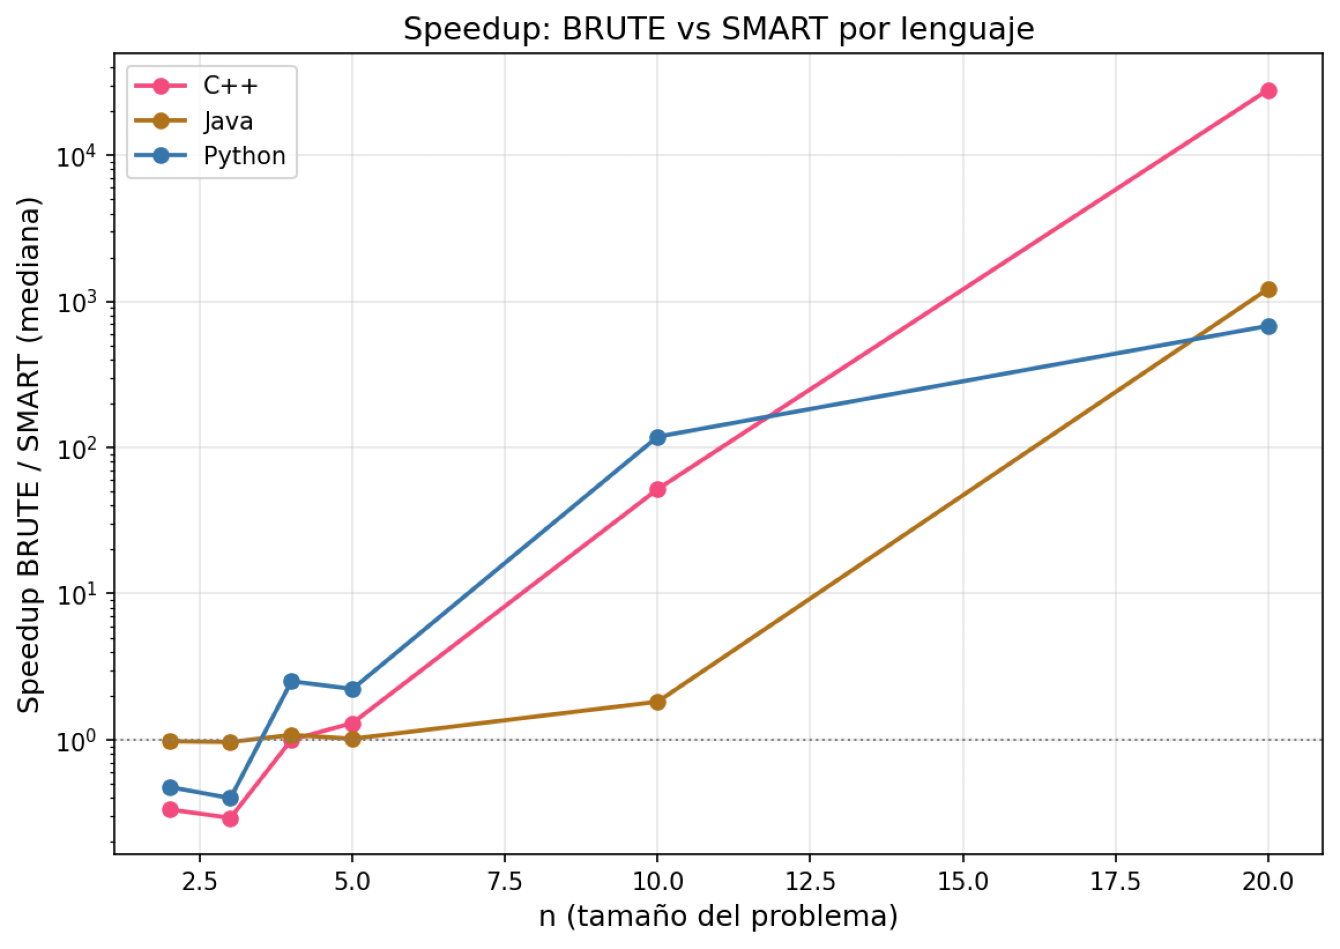
\includegraphics[width=\linewidth]{figuras/brute_vs_smart.pdf}
\end{center}
\end{column}

\begin{column}{0.41\textwidth}

\textbf{Cifras destacadas:}

\smallskip
\begin{block}{SMART vs BRUTE}
\small Speedup $> \mathbf{60\,000\times}$\\
para $n{=}20$, $m{=}80$
\end{block}

\smallskip
\begin{block}{Entre lenguajes (SMART, $n{=}30$)}
\small
\begin{tabular}{lr}
\textbf{C++}    & $18$ ms  \\
\textbf{Java}   & $52$ ms  \\
\textbf{Python} & $1\,150$ ms \\
\end{tabular}\\[2pt]
C++ vs Java: $\approx 3\times$\\
C++ vs Python: $\approx 63\times$
\end{block}

\smallskip
{\footnotesize\textit{Nodos explorados identicos en los 3 lenguajes (37\,854 para $n{=}30$, $m{=}120$).}}

\end{column}
\end{columns}

\end{frame}

% 07_conclusiones.tex — Slide 7: Conclusiones
\begin{frame}{Conclusiones}

\begin{columns}[T]
\begin{column}{0.55\textwidth}

\textbf{Lo aprendido:}
\begin{itemize}
  \item El modelo ILP guia directamente las podas de SMART.
  \item MRV + forward checking reduce el arbol de busqueda de forma exponencial.
  \item Logica identica en 3 lenguajes; solo cambia la velocidad.
\end{itemize}

\smallskip
\textbf{Limitaciones:}
\begin{itemize}
  \item $n \le 50$; instancias \textit{large} ($n{=}100$) intractables.
  \item Sin paralelismo (un solo hilo).
\end{itemize}

\end{column}

\begin{column}{0.42\textwidth}

\begin{block}{Trabajo futuro}
\begin{itemize}
  \item \textbf{Aproximaciones}: local-search de Cygan ($\approx 0.66$).
  \item \textbf{FPT}: parametrizacion por treewidth.
  \item \textbf{Paralelismo}: work-stealing en backtracking.
\end{itemize}
\end{block}

\medskip
\centering
\large
\textbf{3DM es NP-completo,}\\
\textbf{pero las podas importan.}

\end{column}
\end{columns}

\end{frame}


% ---- Backup ----
% 99_backup.tex — Slides de backup para preguntas
\appendix

\begin{frame}{Backup: Tabla de tiempos completa (small suite)}

\begin{center}
\footnotesize
\begin{tabular}{llrrl}
\toprule
Lenguaje & Algoritmo & $n$ & Mediana (ms) & Instancias \\
\midrule
C++     & brute & 5  & 0.006   & 6 \\
C++     & brute & 10 & 0.467   & 25 \\
C++     & brute & 20 & timeout & 25 \\
C++     & smart & 5  & 0.005   & 6 \\
C++     & smart & 10 & 0.011   & 25 \\
C++     & smart & 20 & 0.060   & 25 \\
\midrule
Java    & brute & 10 & 5.932   & 25 \\
Java    & brute & 20 & timeout & 25 \\
Java    & smart & 10 & 3.361   & 25 \\
Java    & smart & 20 & 4.454   & 25 \\
\midrule
Python  & brute & 10 & 24.544  & 25 \\
Python  & brute & 20 & timeout & 25 \\
Python  & smart & 10 & 0.269   & 25 \\
Python  & smart & 20 & 2.725   & 25 \\
\bottomrule
\end{tabular}
\end{center}

{\small Timeout = 30 s (small suite). Valores 5000 ms en CSV corresponden al timeout del script.}

\end{frame}

\begin{frame}{Backup: Correctitud de las 6 implementaciones}

\begin{center}
\begin{tabular}{llrrll}
\toprule
Instancia & $n$ & $m$ & OPT & Acuerdo & Todos \\
\midrule
mini1   & 2 & 3  & 2 & SI & 2 \\
mini2   & 3 & 5  & 3 & SI & 3 \\
noperf  & 3 & 3  & 1 & SI & 1 \\
dense   & 4 & 16 & 4 & SI & 4 \\
empty   & 5 & 0  & 0 & SI & 0 \\
\bottomrule
\end{tabular}
\end{center}

\medskip
\textbf{0 discrepancias de bug} en todas las instancias completadas.\\
Los 6 solvers producen identico $\mathrm{OPT}(I)$ y mismos nodos explorados.

\end{frame}

\begin{frame}{Backup: Gadgets de la reduccion 3-SAT $\le_p$ 3DM}

\textbf{Gadget de variable} $u_i$ con $k_i$ ocurrencias:
\begin{itemize}
  \item Elementos: $\{t^i_p\}_{p=1}^{k_i} \subset X$ (verdadero), $\{f^i_p\} \subset X$ (falso), $\{a^i_p\}\subset Y$, $\{b^i_p\}\subset Z$
  \item Tripletas: $T^i_p = (t^i_p, a^i_p, b^i_p)$ y $F^i_p = (f^i_p, a^i_{p \bmod k_i+1}, b^i_p)$
  \item Lema de consistencia: el matching fuerza O todos $T^i_*$ O todos $F^i_*$
\end{itemize}

\medskip
\textbf{Gadget de clausula} $C_j = (\ell_1 \vee \ell_2 \vee \ell_3)$:
\begin{itemize}
  \item Dos nuevos elementos $c_j \in Y$, $c'_j \in Z$
  \item Tres tripletas-clausula (una por literal); exactamente una puede ser seleccionada
\end{itemize}

\medskip
\textbf{Tamano de la reduccion:} $n = 6q$ elementos por dimension, $m = O(q^3)$ tripletas, construccion en tiempo polinomial.

\end{frame}

\begin{frame}{Backup: Fenomeno Java $>$ C++ para instancias largas}

Para $n{=}50$, $m{=}200$ (instancia \textit{random\_n50\_m200\_s0}):
\begin{itemize}
  \item \textbf{C++ smart}: 39.0 s (38\,944 ms)
  \item \textbf{Java smart}: 29.8 s (29\,843 ms)
  \item \textbf{Python}: timeout en 60 s
\end{itemize}

\medskip
\textbf{Explicacion:}
\begin{itemize}
  \item Mismos nodos explorados (57\,998\,790): logica identica
  \item JIT HotSpot (Temurin-21) con warm-up completo supera GCC~-O2
  \item \texttt{Long.bitCount()} llega al hardware POPCNT igual que C++
  \item JIT hace mejor especulacion de branches en el loop interno
\end{itemize}

\medskip
\small\textit{Este fenomeno esta bien documentado: JIT puede superar AOT en workloads con patrones predecibles y hot loops.}

\end{frame}


\end{document}
